% *******************************************************
% SUPPRESS WARNINGS
% *******************************************************
\RequirePackage{silence}
\WarningFilter{scrbook}{Usage of package `titlesec'}
\WarningFilter{titlesec}{Non standard sectioning command detected}

% \tolerance=1
\emergencystretch=\maxdimen
% \hyphenpenalty=200 % Defined later just before body
\hbadness=10000

% *******************************************************
% DOCUMENT FRONT MATTER START
% *******************************************************
\documentclass[11pt,twoside,openright,titlepage,
  headinclude,footinclude,BCOR=5mm,
  numbers=noenddot,cleardoublepage=empty,
  tablecaptionabove, dottedtoc,
  bibliography=totoc,paper=a4]{scrreprt}
\PassOptionsToPackage{hyphens}{url}
\usepackage[automark]{scrlayer-scrpage}
\usepackage[linktocpage=true]{hyperref}
\usepackage{subfig}
\usepackage[eulerchapternumbers, subfig, beramono, eulermath, pdfspacing]{classicthesis} 
\usepackage{arsclassica}
\usepackage{amsmath}
\usepackage{amssymb}
\usepackage{graphicx}
\usepackage{booktabs}
\usepackage[utf8]{inputenc}
\usepackage[T1]{fontenc}
\usepackage{pdfpages}
\usepackage{titlesec}
\usepackage{titletoc}
\usepackage{longtable} 
\usepackage[norsk,american]{babel}
\usepackage[paperwidth=17cm, paperheight=24cm, margin=2.5cm]{geometry}
\usepackage[cam,a4,center,pdflatex]{crop}
\usepackage{easyReview}
% \usepackage{setspace}

% *******************************************************
% ADDITIONAL PACKAGES
% *******************************************************

% *******************************************************
% REFERENCE PACKAGES
% *******************************************************
  \usepackage[authoryear]{natbib}
  \bibliographystyle{plainnat}

% *******************************************************
% DEFINE VARIABLES
% *******************************************************
\newcommand{\Name}{Raju Rimal}
\newcommand{\Title}{Exploration of Multi-Response Multivariate Methods}
\newcommand{\Location}{\spacedlowsmallcaps{Ås}}
\newcommand{\Year}{2019}
\newcommand{\Month}{Aug}
\newcommand{\Date}{\Year, \Month}
\newcommand{\docsite}{\url{https://therimalaya.github.com/thesis}}
\newcommand{\Subtitle}{}
\newcommand{\email}{\mail{raju.rimal@nmbu.no}}
\newcommand{\homepage}{\url{https://www.mathatistics.com/}}
\newcommand{\Affiliation}{Norwegian University of Life Sciences\\
Faculty of Chemistry, Biotechnology and Food Science\\}
\newcommand{\Faculty}{}
\newcommand{\Group}{}
\newcommand{\alttitle}{Utforskning av multi-respons multivariate metoder}

% *******************************************************
% CUSTOMIZATIONS
% *******************************************************
\newcommand{\mail}[1]{\href{mailto:#1}{\texttt{#1}}}
\titlecontents{part}[0pt]{\pagebreak}{}{\Large\MakeTextUppercase}{}
\titleformat{\part}[display]
  {\normalfont\centering\Large}%
  {\thispagestyle{empty}\partname~\MakeTextUppercase{\thepart}}{1em}%
  {\color{Maroon}\spacedallcaps}
\providecommand{\tightlist}{%
  \setlength{\itemsep}{0pt}\setlength{\parskip}{0pt}}
\DeclareTOCStyleEntry[beforeskip=3pt]{tocline}{section}

\DeclareTOCStyleEntry[numwidth=2em]{tocline}{figure}
\DeclareTOCStyleEntry[numwidth=2em]{tocline}{table}

\titleformat{\section}{\normalfont\large\raggedright}{\thesection}{1em}{}

% *******************************************************
% DOCUMENT BEGIN
% *******************************************************
\begin{document}
\pagenumbering{Roman}
\pagestyle{plain}

% *******************************************************
% Title Front
% *******************************************************
\begin{titlepage}
  \pdfbookmark{Titlepage}{Titlepage}
  \begin{center}
    \large \sffamily
    \bigskip
    {\huge\spacedlowsmallcaps{\Title} \\}
    \bigskip
    {\large{\alttitle}} \\
    \vfill
    {\Large\spacedlowsmallcaps{Philosophiae Doctor (PhD) Thesis}} \\
    \bigskip
    {\Large{\spacedlowsmallcaps\Name}} \\
    \vfill
    {\normalsize \Affiliation}
    \vfill
    {\normalsize \Location (\(\Year\))\\}
    \vfill
              \newcommand{\logowidth}{0.35\linewidth}
          
\includegraphics[width=\logowidth]{Logo1.png} \\
        \vfill
    {\normalsize
      Thesis Number: 2019:76\\
      ISSN:  1894-6402\\
      ISBN:  978-82-575-1636-9\\
    }
  \end{center}
\end{titlepage}

% *******************************************************
% Title Back
% *******************************************************
\thispagestyle{empty}
\hfill \vfill
\noindent
\textit{The goal is to turn data into information, and information into insight.}\\
\spacedlowsmallcaps{- Carly Fiorina, former CEO of Hewlett-Packard}
\vfill
\noindent
{\textbf{Supervisors:}} \\
Professor \textit{Solve Sæbø}\\
Prorector of Education\\
Norwegian University of Life Sciences\\
Ås, Norway\\
\medskip\\
Associate Professor \textit{Trygve Almøy}\\
Norwegian University of Life Sciences\\
Faculty of Chemistry, Biotechnology and Food Science\\
Ås, Norway\\
\medskip\\
\bigskip \\
\noindent
\textit{\Title} \\
{\spacedlowsmallcaps{PhD Thesis, \Date\,\, \textcopyright\, \Name}} \\
\bigskip \\
\noindent{\spacedlowsmallcaps{Website}}: \\
\docsite \\
\medskip
\noindent{\spacedlowsmallcaps{E-mail}}: \\
\email
\vspace{1cm}
\hrule
\bigskip
\noindent This thesis is prepared with \texttt{ArsClassica} {\LaTeX} template with \texttt{pandoc} and r-package \texttt{bookdown}.
% \begin{flushright}source: \url{https://therimalaya.github.com/thesis}\end{flushright}

% *******************************************************
% ABSTRACT
% *******************************************************

% *******************************************************
% SUMMARY
% *******************************************************
\begingroup
%\pdfbookmark{Summary}{Summary}
\addchap{Summary}
A linear regression model defines a linear relationship between two or
more random variables. The random variables that depend on other random
variables are often called response variables and the independent random
variables are called predictor variables. In most cases not all
variation is relevant for regression, i.e.~only a certain amount of the
variation in the predictors is relevant and only so for a part of the
variation in the response. This leads to a reduction of the linear
regression model where one can imagine a subspace of the space spanned
by the predictor variables that contains all the relevant information
for a subspace of the space spanned by the response variables.

In this thesis we attempt to compare some new methods which are based on
the envelope model and some established methods such as principal
components regression (PCR) and partial least squares regression (PLS).
The comparison tests these methods on their performance of producing
minimum prediction and estimation error while modelling data simulated
with specifically designed properties. For the simulation we have also
created an R-package called \texttt{simrel} with a web interface.

A simulation model for a multi-response multivariate linear model, on
which the simulation tool is based, is discussed in the first paper.
This paper prepares a basic foundation for the simulations with the
concept of reduction of regression models. The second paper discusses
the similarities of the envelope, PCR and PLS population models. This
paper compares the prediction performance of several multivariate
methods using a model with a single response.

The final two papers make an extensive investigation evaluating the
prediction and estimation performance of established (PCR, PLS1 and
PLS2) and newly developed envelope based (Xenv and Senv) methods.
Unsurprisingly the study found that not one method dominates in all
situations, but their performance depend on the properties of the data
they model. However, the envelope based methods have shown remarkable
performance in many cases, both in prediction and estimation. The study
also recommend researchers to use and evaluate the envelope methods.


\KOMAoptions{open=left}
\begin{otherlanguage}{norsk}
%\pdfbookmark{Sammendrag}{Sammendrag}
\addchap{Sammendrag}
En lineær regresjonsmodell definerer et lineært forhold mellom to eller
flere tilfeldige variabler. De tilfeldige variablene som er avhengige av
andre tilfeldige variabler, kalles ofte responsvariabler, og de
uavhengige tilfeldige variablene kalles prediktorvariabler. I de fleste
tilfeller er ikke all variasjon relevant for regresjon, dvs. bare en
viss mengde variasjonen i prediktorene er relevante, og bare for en del
av variasjonen i responsen. Dette fører til en reduksjon av den lineære
regresjonsmodellen der man kan forestille seg et underrom av rommet som
spennesut av prediktorvariablene som inneholder all relevant informasjon
for et underrom av rommet spent ut av responsvariablene.

I denne avhandlingenprøver vi å sammenligne noen nye metoder som er
basert på Envelopemodellen og noen etablerte metoder som principal
komponent regresjon (PCR) og partiell minste kvadraters regresjon (PLS).
Sammenligningen tester disse metodene på deres ytelse til å produsere
minimum prediksjon- og estimeringsfeil, mens modelleringsdata simuleres
med spesielt designede egenskaper. For simuleringen har vi også laget en
R-pakke kalt \texttt{simrel} med et webgrensesnitt.

En simuleringsmodell for multirespons, multivariat lineær modell, som
simuleringsverktøyet bygger på, diskuteres i den første artikkelen.
Denne artikkelen utarbeider et grunnleggende fundament for simuleringene
basert på konseptet om reduksjon av regresjonsmodeller. Den andre
artikkelen diskuterer likhetene i Envelope-, PCR- og
PLS-populasjonsmodellene. Denne artikkelen sammenligner
prediksjonsytelsen til flere multivariate metoder ved bruk av en modell
med en enkelt respons.

De to siste artiklene gir en grundig evaluering av prediksjons- og
estimeringsegenskapene til etablerte metoder (PCR, PLS1 og PLS2) og
nyutviklede envelope-baserte metoder (Xenv og Senv). Ikke uventet fant
studien at det ikke finnes en enkelt metode som dominerer i alle
situasjoner, men resultatene deres avhenger av egenskapene til dataene
de modellerer. Imidlertid har envelope-baserte metoder vist
bemerkelsesverdig resultater i mange tilfeller, både når det gjelder
prediksjon og estimering. Studien anbefaler også forskere å bruke og
evaluere envelope-metodene.

\end{otherlanguage}
\KOMAoptions{open=right}
\endgroup

% *******************************************************
% ACKNOWLEDGMENT
% *******************************************************
%\pdfbookmark{Acknowledgments}{Acknowledgments}
\begingroup
\cleardoublepage
\addchap{Acknowledgment}
First and foremost, I am indebted to my supervisor Solve Sæbø who picked
me up from nowhere and brought me into a scientific community by giving
me a chance to pursue this degree. His inspiration and encouragement
have been an essential element in the course of this journey. I am
grateful to my co-supervisor Trygve Almøy for being a mentor, a friend,
a colleague, and a guardian and guiding and supporting me throughout
this period. He has always been there for me with my frustration and
excitement.

I am forever grateful to my father Narayan Prasad Rimal and mother
Bhagawati Rimal for their continuous support and encouragement. Their
belief in me and push for my education have shined the light in my hard
and easy times. I am also thankful to my dear wife Junali Chhetri who
has inspired me every step of my life and help me to better understand
myself. And of course, a thank goes to my beloved son Nirvan Rimal who
has understood my busy time during this study.

I would also like to thank Professor Inge Helland for his insight,
suggestion and comment on many mathematical problems on various
statistical methods presented in the thesis.

Last, but importantly, my thank goes to the Biostatistics group with
whom I have collected beautiful memories. Thanks to all the members of
the group from past and present who have always made my stay at NMBU
happy, festive and full of joy.

\endgroup

% *******************************************************
% PREFACE
% *******************************************************
%\pdfbookmark{Preface}{Preface}
\begingroup
\cleardoublepage
\addchap{Preface}
This thesis is a part of Doctor of Philosophy (PhD) study. The first
part of the thesis constitute a gentle introduction to the objective of
the study and some of its background. This is followed by the summary of
individual research paper on which this thesis is based on. The
discussion section tries to bind the finding from theses papers. The
final chapter will discuss the limitations and future prospect of the
study. The second part contains all the papers attached.

An R-package called \texttt{simrel} is available as part of the first
paper included in this thesis. The package lets users simulated data
from a multi-response linear model. The package can be installed from
R-package repository CRAN or from GitHub. In addition, a web application
that gives users a graphical user interface for the package is also
available from GitHub. All the results and the documentations of the
research can be reproduced from the codes in GitHub repository with
software and packages required installed. In addition, one can use
docker image together with the code for reproducing the thesis together
with all included papers. All related resources are listed in the final
chapter.

\endgroup

% *******************************************************
% INCLUDE ANYTHING BEFORE
% *******************************************************

% *******************************************************
% Contents
% *******************************************************
\cleardoublepage
\phantomsection
\pdfbookmark{\contentsname}{tableofcontents}
\setcounter{tocdepth}{1}
\begingroup 
  \let\clearpage\relax
  \let\cleardoublepage\relax
    \tableofcontents
\endgroup
\markboth{\spacedlowsmallcaps{\contentsname}}
{\spacedlowsmallcaps{\contentsname}} 

\begingroup

% Number the sections
\setcounter{secnumdepth}{-\maxdimen} % remove section numbering

\listoffigures
\vfill
\endgroup

\begingroup 
  \let\clearpage\relax
  \let\cleardoublepage\relax
\endgroup

\cleardoublepage

% *******************************************************
% BODY START
% *******************************************************

\pagenumbering{arabic}
\hyphenpenalty=200

\pagestyle{scrheadings} 
\automark[chapter]{chapter}
%\automark[section]{}
%\doublespacing

\hypertarget{introduction}{%
\chapter{Introduction}\label{introduction}}

Rapid development in technology and computational power have resulted in heaps of data. Extracting information from this chaotic heaps of data has become another problem. Many statistical and machine learning tools are devised for this purpose, most of which focus to identify the relationships between different variables. A linear relationship is the most common assumption. This thesis confined itself in the exploration of linear relationships, where a set of independent variables, called predictor variables, affect another set of dependent variables, called response variables. The space spanned by the columns of predictors and responses are termed \emph{predictor space} and \emph{response space}, respectively.

Many projection-based statistical methods such as Principal Components Regression (PCR), Partial Least Squares (PLS) Regression and some variants of Envelopes only consider a subspace of predictor space relevant for defining the linear relationship between the predictors and the response(s). This brings us to the concept of relevant and irrelevant space introduced by \citet{Naes1985}. The relevant space can be described as the subspace that contains all the required information to define the relationship between the predictors and the response in a model. The irrelevant space, on the other hand, does not contain any information regarding this relationship.

Latent components corresponding to predictor variables, which we will refer to as ``predictor components'', are linear combinations of the predictor variables. \citet{Naes1985} and later \citet{helland1990partial}, \citet{naes1993relevant} and \citet{Helland1994b} have defined a set of predictor components as irrelevant components if they have no correlation with the response variables and the relevant part. Using only a subset of the latent components for modeling, is often termed as ``dimension reduction''. Methods like PCR, PLS and many other variants of PLS has leveraged this concept and are serving as prime tools in many disciplines, most notably in chemometrics.

Relatively new methods based on the concept of ``envelopes'' introduced by \citet{Cook2007a}, more specifically envelope in predictor variable (Xenv), have also used this concept of dimension reduction. In addition, envelope in response variable (Yenv) and simultaneous envelope in predictor and response (Senv) have extended the concept of relevant and irrelevant space to the response space as well, which they referred to as material and immaterial part. These methods are discussed in \protect\hyperlink{background}{Background} section.

Despite having similar underlying population model, these methods estimate the model parameters differently. Model parameters are the unknowns, which help to define a complex relationships between the variables. Regression coefficient vector \((\beta)\) in \eqref{eq:linear-reg-model} is an example of a model parameter. All methods use data to estimate these parameters. So, the properties of a dataset affect the estimation and consequently the prediction performance of the methods. Evaluation of these methods is essential to understand how they interact with various properties of the data. This thesis will explore some of these methods and assess their estimative and predictive strength and weaknesses through both simulated and real datasets.

This exploration adds a reference for researchers to motivate them for using different methods based on the properties of the data they are working on. This study is exploratory in nature where we assess and compare different multi-response multivariate methods, but most importantly study their interaction with the properties of the data. The properties include the correlation between predictor variables, the position of principal components of predictor variables (predictor components) that are relevant for certain principal components of the response variables (response components), the amount of correlation between the response variables and the number of predictor variables. The effect of the correlation structure of the response matrix is less explored and it is expected to shed some light on how similar and how different the methods are in terms of modelling this structure. In order to simulate data with these properties varying at different levels, we have created an R-package called \texttt{simrel}, which is an extension of the previous version introduced by \citet{saebo2015simrel} to incorporate multiple responses.

\hypertarget{background}{%
\chapter{Background}\label{background}}

This section discusses the relevant topics that have been used in the included papers.

\hypertarget{multivariate-linear-regression-model}{%
\section{Multivariate Linear Regression Model}\label{multivariate-linear-regression-model}}

The joint normal distribution of a random variable-vector \(\mathbf{y}\) of \(m\) response variables with mean of \(\boldsymbol{\mu}_y\) and another random variable-vector \(\mathbf{x}\) of \(p\) predictor variables with mean \(\boldsymbol{\mu}_x\) as,

\begin{equation}
\begin{bmatrix}
  \mathbf{y}\\
  \mathbf{x}
\end{bmatrix} \sim
\mathsf{N}
\begin{pmatrix}
  \begin{bmatrix}
    \boldsymbol{\mu_y}\\
    \boldsymbol{\mu_x}
  \end{bmatrix},
  \begin{bmatrix}
    \boldsymbol{\Sigma_{yy}} & \boldsymbol{\Sigma_{yx}} \\
    \boldsymbol{\Sigma_{xy}} & \boldsymbol{\Sigma_{xx}}
  \end{bmatrix}
\end{pmatrix}
\label{eq:linear-model}
\end{equation}
where \(\boldsymbol{\Sigma}_{xx}\) and \(\boldsymbol{\Sigma}_{yy}\) are the variance-covariance matrices of \(\mathbf{x}\) and \(\mathbf{y}\), respectively, and \(\boldsymbol{\Sigma}_{xy} = \boldsymbol{\Sigma}_{yx}^t\) is the covariances between them.

A model that linearly relates \(\mathbf{x}\) and \(\mathbf{y}\) through regression coefficient vector \(\boldsymbol{\beta}\) is often written as,

\begin{equation}
\mathbf{y} = \boldsymbol{\mu}_y + \boldsymbol{\beta}^t\left(\mathbf{x} - \boldsymbol{\mu}_x\right) + \boldsymbol{\varepsilon}
\label{eq:linear-reg-model}
\end{equation}
where \(\boldsymbol{\varepsilon} \sim \textsf{N}\left(\mathbf{0}, \boldsymbol{\Sigma}_{y|x}\right)\)

We can write the regression coefficient \(\boldsymbol{\beta} = \boldsymbol{\Sigma}_{xx}^{-1}\boldsymbol{\Sigma}_{xy}\) in terms of the covariance matrices. A complete simulation of this model requires to specify \(1/2(p+m)(p+m+1)\) unknowns.

With a transformation defined as \(\mathbf{z} = \mathbf{Rx}\) and \(\mathbf{w} = \mathbf{Qy}\) with \(\mathbf{R}_{p\times p}\) and \(\mathbf{Q}_{m\times m}\) as random orthogonal rotation matrices, model \eqref{eq:linear-model} can be rewritten as,

\begin{align}
  \begin{bmatrix}\mathbf{w} \\
  \mathbf{z}\end{bmatrix}  & \sim N \left(\boldsymbol{\mu}, \boldsymbol{\Sigma}\right)
  = N \left(
    \begin{bmatrix}
      \boldsymbol{\mu}_w \\ \boldsymbol{\mu}_z
    \end{bmatrix},
    \begin{bmatrix}
      \boldsymbol{\Sigma}_{ww} & \boldsymbol{\Sigma}_{wz} \\
      \boldsymbol{\Sigma}_{zw} & \boldsymbol{\Sigma}_{zz}
    \end{bmatrix} \right) \nonumber \\
  &= N \left(
    \begin{bmatrix}
      \boldsymbol{Q\mu}_y \\
      \boldsymbol{R\mu}_x
    \end{bmatrix},
    \begin{bmatrix}
      \boldsymbol{Q\Sigma}_{yy}\boldsymbol{Q}^t & \boldsymbol{Q\Sigma}_{yx}\mathbf{R}^t \\
      \boldsymbol{R\Sigma}_{xy}\boldsymbol{Q}^t & \boldsymbol{R\Sigma}_{xx}\mathbf{R}^t
    \end{bmatrix}
  \right)
  \label{eq:latent-model}
\end{align}

Since both \(\mathbf{Q}\) and \(\mathbf{R}\) are orthonormal matrices, i.e., \(\mathbf{Q}^t\mathbf{Q} = \mathbf{I}_m\) and \(\mathbf{R}^t\mathbf{R} = \mathbf{I}_p\), the inverse transformation can be defined as,

\begin{equation}
  \begin{matrix}
    \boldsymbol{\Sigma}_{yy} = \mathbf{Q}^t \boldsymbol{\Sigma}_{ww} \mathbf{Q} &
    \boldsymbol{\Sigma}_{yx} = \mathbf{Q}^t \boldsymbol{\Sigma}_{wz} \mathbf{R} \\
    \boldsymbol{\Sigma}_{xy} = \mathbf{R}^t \boldsymbol{\Sigma}_{zw} \mathbf{Q} &
    \boldsymbol{\Sigma}_{xx} = \mathbf{R}^t \boldsymbol{\Sigma}_{zz} \mathbf{R}
  \end{matrix}
  \label{eq:cov-yx-wz}
\end{equation}

Here, \(\boldsymbol{\Sigma_{zz}}\) and \(\boldsymbol{\Sigma_{ww}}\) are diagonal matrices of eigenvalues corresponding to predictors and responses respectively. Following the concept of relevant components \(\boldsymbol{\Sigma}_{wz}=\boldsymbol{\Sigma}_{zw}^t\) has non-zero elements for relevant components. With some random orthogonal rotation matrices \(\mathbf{R}\) and \(\mathbf{Q}\), which can be easily generated, the unknowns required for simulation may drastically decrease. Following the idea from \citet{saebo2015simrel}, Paper I uses exponential decay of eigenvalues, as in \eqref{eq:exp-decay}, that fills the diagonals of \(\boldsymbol{\Sigma}_{zz}\) and \(\boldsymbol{\Sigma}_{ww}\). Here the decay factor \(\gamma\) controls the multicollinearity such that a higher value of gamma corresponds to high multicollinearity.

\begin{equation}
\lambda_i = e^{-\gamma(i - 1)}, \gamma >0 \text{ and } i = 1, 2, \ldots, p
\label{eq:exp-decay}
\end{equation}

A thorough discussion on the reparameterization of a linear model to simulate data by the concept of ``relevant components'' can be found in Paper I. The following subsection discusses the concept of relevant components in brief.

\hypertarget{relevant-space-and-relevant-components}{%
\section{Relevant Space and Relevant Components}\label{relevant-space-and-relevant-components}}

In the model \eqref{eq:linear-model}, not all information in \(\mathbf{x}\) is relevant for \(\mathbf{y}\) and not all variation in \(\mathbf{y}\) is explainable or non-redundant. We can refer to the space ``with information'' as relevant (informative) space and the rest as irrelevant (uninformative) space. \citet{Naes1985} introduced the definition of relevant space as the decomposition of the predictor space into two orthogonal subspaces: the relevant and the irrelevant space. Additionally, a set of predictor components defined as irrelevant components do not have any correlation with the response and the relevant part of the data. The relevant components, on the other hand, contains all the required information to explain the variation in the response \(\mathbf{y}\). Multivariate methods such as Principal Components Regression (PCR) and Partial Least Squares (PLS) Regression uses the eigenvectors to span the relevant and irrelevant spaces. Here, we refer the eigenvectors that span the relevant space as \emph{relevant eigenvectors}. The concept was further discussed and developed by \citet{helland1990partial}, \citet{naes1993relevant} and \citet{Helland1994b}. However, all these studies have discussed the separation of relevant and irrelevant space only in the predictor space.

More recently, various estimators \citep{cook2010envelope, cook2013envelopes, cook2015simultaneous} based on a so-called ``envelope'' \citep{Cook2007a} have used and extended the concepts of the separation of relevant and irrelevant spaces to the response space as well. The relevant and irrelevant spaces are referred to as material and immaterial spaces in their literature (Figure \ref{fig:relspace-plot}). The envelope methods use ``envelope'', a linear combination of relevant eigenvectors \citep{cook2018envelope}, to span the relevant space.



\begin{figure}[!htb]
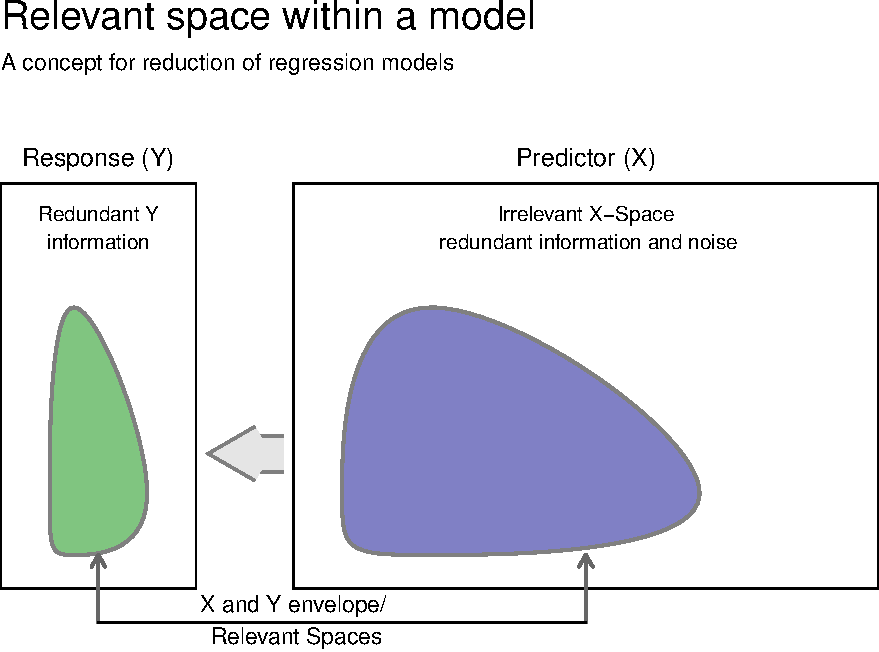
\includegraphics[width=1\linewidth]{Thesis_files/figure-latex/relspace-plot-1} \caption[A heuristic illustration of relevant and irrelevant spaces]{A heuristic illustration of relevant and irrelevant spaces in a response space and a predictor space}\label{fig:relspace-plot}
\end{figure}

To elaborate on the concept of relevant components and how they interact with other properties and influence the prediction of methods, let us consider an example. Assume a single response model with 10 predictor variables where the information contained in these 10 predictors can be completely explained by four principal components of \(\Sigma_{xx}\), the variance-covariance matrix of the predictor (\(\mathbf{x}\)). These four components are the relevant components. Consider two cases:

\begin{description}
\tightlist
\item[Case 1 (Figure \ref{fig:relcomp-example}, left):]
The position of these relevant components are 1, 2, 3 and 4. The eigenvalues of \(\Sigma_{xx}\) decay slowly, i.e.~low multicollinearity. Here, the relevant components from 1 to 4 have large variation, so that, most methods easily extract the information and fit the model quite accurately.
\item[Case 2 (Figure \ref{fig:relcomp-example}, right):]
The position of the relevant components are at 5, 6, 7 and 8. The eigenvalues of \(\Sigma_{xx}\) decay rapidly, i.e.~high multicollinearity. Here the relevant components from 5 to 8 have small variation, so that, it is difficult for most methods to extract the information and fit the model.
\end{description}



\begin{figure}[!htb]
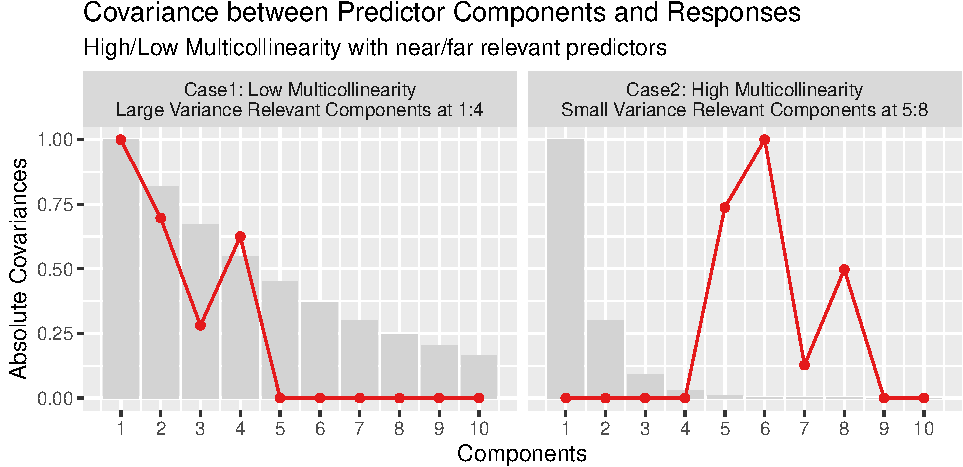
\includegraphics[width=1\linewidth]{Thesis_files/figure-latex/relcomp-example-1} \caption[Relevant Components and Multicollinearity]{Relevant components at two different set of positions and two different levels of multicollinearity. The points represents the correlation of predictor components and the response variable. The grey bars are the eigenvalues of \(\boldsymbol{\Sigma}_{xx}\).}\label{fig:relcomp-example}
\end{figure}

Further, PCR and PLS regression are used with the data simulated from these two cases. Also, leave-one-out cross-validation validates their prediction performance, and the root mean squares error of prediction measures their prediction error (Figure \ref{fig:rmsep-plot}).

Different methods target these cases differently. For example, PCR tries to capture maximum variation in \(\mathbf{x}\) through principal components, so it starts reducing its prediction error only after including the relevant components. For this method, in the first case, prediction error starts decreasing from the first component on, and stabilize after the fourth component while in the second case, prediction error only starts decreasing after the fifth component. This method requires all four relevant components to get the minimum prediction error. Partial Least Square Regression (PLS), on the other hand, is motivated to maximize the covariance between the predictors and the response. We can see a significant decline of prediction error after the first relevant components is included but it uses fewer components to get the minimum prediction error than PCR in both cases. \citet{Helland1994b} has shown a similar result and shown that the relevant components with small variation make the prediction difficult.

\begin{figure}[!htb]
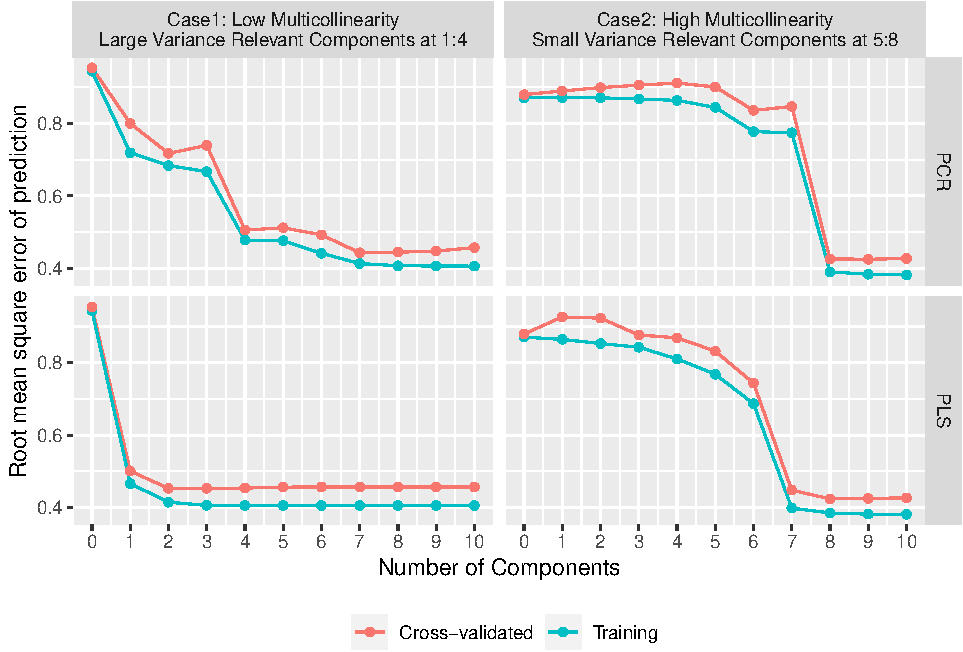
\includegraphics[width=1\linewidth]{Thesis_files/figure-latex/rmsep-plot-1} \caption[]{Root mean square error of cross-validation from PCR and PLSR}\label{fig:rmsep-plot}
\end{figure}

The concept of relevant components can also be extended to the response such that a subspace contains the information relevant for a model. The concept is implemented in the simultaneous envelope \citep{cook2015simultaneous} and the response envelope \citep{cook2010envelope} methods.

\hypertarget{simulation}{%
\section{Simulation}\label{simulation}}

Random variables are the basic components of a complex model and a stochastic simulation. These random variables can be generated on a computer by sampling and manipulating uniform random variables \(U(0, 1)\) which requires random numbers. Although computers can not generate truly random numbers, it can, however, generate pseudo-random numbers. These numbers appear as random numbers but they are completely deterministic. Since they are deterministic, any experiment performed using these numbers can be repeated exactly \citep{jones2014introduction}. We can use these uniform random variables to create other random variables that follow a certain distribution. Standard Normal Distribution is a common one and is used in many statistical simulations including the tool discussed in paper I. Given that we can simulate a standard normal variable \(\mathbf{z}\), one can obtain any normal distribution with arbitrary mean \(\mu\) and variance \(\sigma^2\) as \(\mu + \sigma Z\). Here, we can control the parameters \(\mu\) and \(\sigma\).

Simulation refers to generating data from a known underlying population structure. Controlling the properties of the population is vital in the simulation. This enables researchers and users to use data for comparison of methods, assessing new methodology, testing theory and evaluating algorithms. Such data can also be used for educational purposes.

All the research studies in this thesis have used an R-package called \texttt{simrel} for simulating multi-response linear model data (paper I). The simulation tool is general purpose in nature and has a limited number of parameters that controls the essential properties of the population. It is flexible and enables users to simulate data with a wide range of properties. Some of these properties include the level of correlation between the predictors (\texttt{gamma}) and responses (\texttt{eta}) through exponential decay factor as in \eqref{eq:exp-decay}. The position of the relevant components (\texttt{relpos}), the number of predictor variables (\texttt{p}) and the number of response variables (\texttt{m}) can also be controlled during the simulation.

\hypertarget{estimation-and-prediction}{%
\section{Estimation and Prediction}\label{estimation-and-prediction}}

Measures such as mean and standard deviation for a population are usually referred to as parameters of the population. A model as in \eqref{eq:linear-reg-model}, which expresses the relationship between \(\mathbf{x}\) and \(\mathbf{y}\) in the population, uses parameters such as the error variance and regression coefficients. Usually, due to the lack of known population distribution, the values of these parameters are calculated using a sample collected from the population. The process of determining the value of certain parameters is called estimation. The estimated parameter values from any two samples are different. A method for estimation is considered better if the expected squared difference between the estimated and true value is small and has small variance. The goodness of estimation method depends on the nature of the data. Estimation error with true and estimated regression coefficient \(\boldsymbol{\beta}\) and \(\boldsymbol{\widehat{\beta}}\) respectively, can be defined as in \eqref{eq:est-error}.

\begin{equation}
\text{Estimation Error} = \mathsf{E}\left[
  \left(\boldsymbol{\beta} - \hat{\boldsymbol{\beta}}\right)^t 
  \left(\boldsymbol{\beta} - \hat{\boldsymbol{\beta}}\right)
\right]
\label{eq:est-error}
\end{equation}

A fitted or trained model is mostly used for prediction. Prediction refers to determining the value of the response for a new set of predictors, which were not used to train the model. Most studies under ``data science'' field are targeted for better prediction. Most comparisons in this thesis evaluate the prediction performance of the multivariate methods using the prediction error measured as in \eqref{eq:pred-error}.

\begin{equation}
\text{Prediction Error} = \mathsf{E}\left[
  \left(\boldsymbol{\beta} - \hat{\boldsymbol{\beta}}\right)^t
  \boldsymbol{\Sigma}_{xx}
  \left(\boldsymbol{\beta} - \hat{\boldsymbol{\beta}}\right)
\right] + \boldsymbol{\Sigma}_{y|x}
\label{eq:pred-error}
\end{equation}

From \eqref{eq:est-error} and \eqref{eq:pred-error}, we can see that the prediction errors are influenced by the covariance of the predictors directly, while estimation error is not. In the case of multicollinear predictors, estimation error can be huge, while due to the scaling of the covariation of predictors, the prediction error can still be small. A good estimation can give a proper and trustworthy idea about the relation between certain predictor variation with a certain response variable. This is important in policymaking, academic researches and to understand the relationships when developing new models. Prediction, on the other hand, is widely used from weather forecasting, economic forecasting, prediction in production and sales, and many more.

\hypertarget{multivariate-methods}{%
\section{Multivariate Methods}\label{multivariate-methods}}

Various multivariate methods such as ordinary least squares (OLS), principal components regression (PCR), partial least squares (PLS) regression and envelope methods are used for comparative studies included in this thesis. All of these methods except OLS use the concept of relevant space and the reduction of the regression model. Here we will refer PLS2, which models all the response variables together, as PLS and PLS1, which models each responses separately, as PLS1.

\hypertarget{methods-based-on-envelope-model}{%
\subsection{Methods based on Envelope Model}\label{methods-based-on-envelope-model}}

Three different methods based on envelopes are also included for comparison. \citet{Cook2007a} defined envelope as the smallest subspace that includes the span of true regression coefficients and developed various estimators based on the concept of the envelope through various subsequent papers. Response envelope (Yenv) \citep{cook2010envelope} performs dimension reduction only in the response space while Predictor envelope (Xenv) \citep{cook2013envelopes} performs dimension reduction only in the predictor space. The simultaneous envelope (Senv) \citep{cook2015simultaneous} performs dimension reduction on both predictor and response space simultaneously. If all the possible components (latent dimension) are included in these methods, the results are equivalent to OLS regression. The comparisons of these envelope methods together with PCR and PLS in the third and fourth paper have shown encouraging results for envelope methods in both easy and difficult cases.

\hypertarget{pls-and-its-derivatives}{%
\subsection{PLS and its derivatives}\label{pls-and-its-derivatives}}

Since the PLS method has been both popular and productive in fields like chemometrics, its development has progressed quickly over time through the formulation of various derivatives. CPLS and CPPLS are among them which combines PLS and canonical correlation analysis (CCA) and give a joint framework for classification and regression \citep{indahl2009canonical}. Paper-I has made some basic comparison of these methods for their predictive ability. More recently, \citet{helland2012near}{]} introduced the Bayes PLS method. The method only works with a single response model and has shown promising results compared to other methods in Paper-II.

\citet{WENTZELL2003257} has assembled many comparisons made on PCR and PLS where they conclude that PLS has not shown a clear advantage over PCR over predictive ability in most studies, but uses fewer components than PCR. Many studies are available comparing PCR, PLS and their derivatives. However, there are not any studies to date which have made any empirical comparisons of the newly developed \emph{envelope} based methods using real and simulated data with these more established methods.

Details on each of these methods can be obtained from the corresponding references.

\hypertarget{experimental-design}{%
\section{Experimental Design}\label{experimental-design}}

In all the post hoc comparisons, simulation parameters are considered as independent variables (factors), and the prediction- and estimation errors are considered as outcome variables (responses). Factorial Design is implemented as an experimental design which allowed us to compare all possible combination of different factor levels. For example, the factorial design used throughout the third and fourth paper, shown in Figure \ref{fig:design-plot}, has four factors: a) Number of predictor variables (\texttt{p}) with two levels, b) level of multicollinearity (\texttt{gamma}) with two levels, where higher value represents a higher level of multicollinearity, c) position index of relevant predictor components (\texttt{relpos}) and d) the level of collinearity in response (\texttt{eta}), with four levels where higher value represents a higher correlation between the response variables. The combination of these factors has created 32 unique designs which are then used for simulating data with those particular properties. Such data, with all possible combination of these properties, have made both thorough and rigorous comparison possible.



\begin{figure}[!htb]
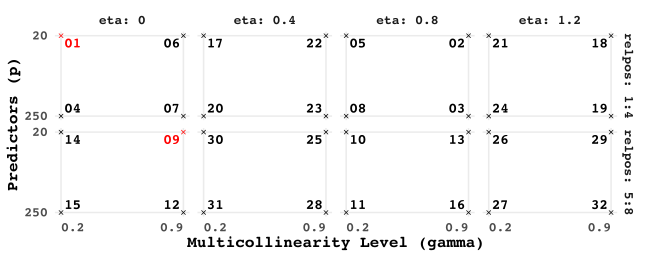
\includegraphics[width=1\linewidth]{Thesis_files/figure-latex/design-plot-1} \caption{An example of a factorial design used in the third and fourth paper.}\label{fig:design-plot}
\end{figure}

Let us dig a little deeper to understand how these simulation parameters are tied with the properties of the simulated data. As an example, let us take Design 1 and Design 9 of Figure \ref{fig:design-plot} where data simulated with Design 1 have low multicollinearity and the position index of relevant components are 1, 2, 3, 4, while Design 9 have high multicollinearity and the position index of relevant components are 5, 6, 7, 8. With other factors or properties of the data being the same for both, the difference in these two designs help us to analyse the interaction between the multicollinearity in the data and the position of relevant components on, for instance, prediction performance of the methods.



\begin{figure}[!htb]
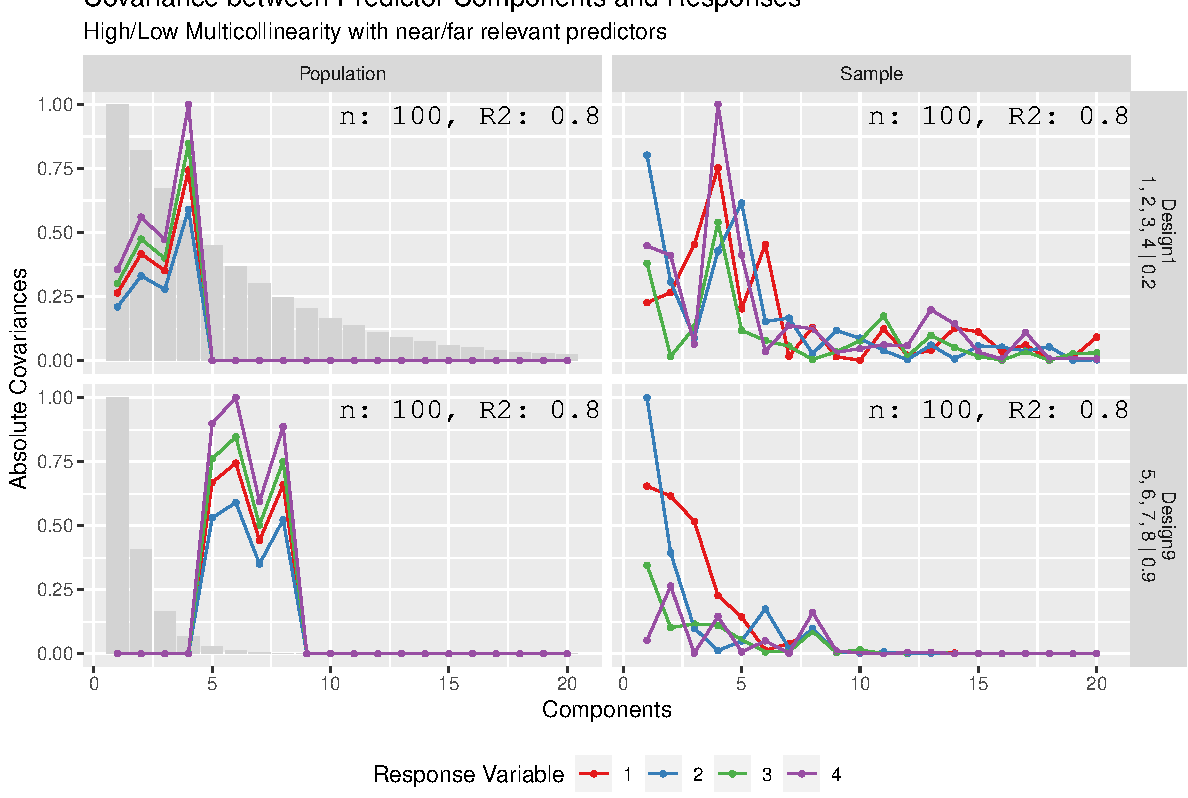
\includegraphics[width=1\linewidth]{Thesis_files/figure-latex/cov-plot-1} \caption{\emph{Design 1}: Relevant components have large variation, \emph{Design 9}: irrelevant components have large variation and relevant components have small variation.}\label{fig:cov-plot}
\end{figure}

Figure \ref{fig:cov-plot} (top-row) shows the scaled covariance between the predictor components and the response variables for Design 1. Here the relevant components with larger variation (due to low multicollinearity) simulate data that are easier to model by most methods. Figure \ref{fig:cov-plot} (bottom-row) for Design 9 shows that the relevant components at position 5, 6, 7, 8 have small variation and irrelevant components at position 1, 2, 3, 4 have large variation. This design simulates data that are difficult to model by most methods. The population covariances in the figure give clear and distinct relationship, while the sample covariances give a somewhat rough approximation of the population.

\hypertarget{analysis-of-variance}{%
\section{Analysis of Variance}\label{analysis-of-variance}}

The analysis in these studies have used various exploratory plots of prediction error, estimation error and the number of components used by different methods. Also, visualizations from principal components analysis (PCA) have been used on these errors. Besides, a more formal analysis is made using analysis of variance (ANOVA). ANOVA allowed us not only to understand the effect of various properties of data controlled by the simulation parameters but also analyses the effect of the interaction of these properties with the methods. The third and fourth paper use multivariate analysis of variance (MANOVA) to analyze the effect on four response variables.

MANOVA is the multivariate counterpart of the ANOVA where various test statistic are used, such as Wilks' Lambda, Lawley-Hotelling trace, Pillai trace and Roy's largest root. All of these methods use the within \((\mathbf{E})\) and between \((\mathbf{H})\) sum of squares and the cross products matrices. All four test statistic are nearly equivalent for large sample size \citep{johnson2018applied}. In our studies, Pillai trace is used, which is defined as,

\begin{equation}
\text{Pillai statistic} = \text{tr}\left[(E + H)^{-1}H\right] = \sum_{i=1}^{m}{\frac{\nu_i}{1+\nu_i}}
\label{eq:pillai}
\end{equation}
where, \(\nu_i\) represents the eigenvalues corresponding to \(\mathbf{E^{-1}H}\).

\hypertarget{paper-summary}{%
\chapter{Paper Summary}\label{paper-summary}}

\hypertarget{paper-1-a-tool-for-simulating-multi-response-linear-model-data}{%
\section{Paper 1: A Tool for Simulating Multi Response Linear Model Data}\label{paper-1-a-tool-for-simulating-multi-response-linear-model-data}}

As an extension of \citet{saebo2015simrel} to simulate linear model data with multiple response variables, this paper discusses the simulation model, the strategy for simulation, and compares some multivariate methods using simulated data. Additionally, it includes an R-package called \texttt{simrel} that is built based on the mathematical formulation discussed in the paper.

The simulation of the linear model discussed here is based on the concept of the relevant components. A subspace of the predictor space, which is relevant for a subspace of response space, is the basis of the simulation tool. These subspaces are assumed to be spanned by a subset of respective latent components. The simulation strategy started with identifying the covariance between these components that satisfy the user's condition for the data, i.e.~the simulation parameters. A covariance structure of the latent space is then created which is rotated by an arbitrary orthogonal rotation matrix to obtain the population covariance structure of the simulated data. Data is then sampled from a normal distribution with the constructed covariance structure. The tool also provides mathematically computed properties of the data such as true regression coefficient, minimum model error, coefficient of determination and the predictor variables relevant for a given response.

In addition to the mathematical formulation for simulation, the study compares some multivariate methods including OLS, PCR, PLS and Envelope using two simulation examples. It has included some derivatives of PLS such as PLS1, PLS2, CPLS and CPPLS and some methods based on envelope estimation such as Xenv, Yenv and Senv. The first example has three relevant response components rotated into five response variables. Additionally, four simulation designs were constructed using factorial design with low and high multicollinearity interacting with low and high noise levels. The simultaneous envelope (Senv) method has achieved the smallest prediction error with a smaller number of components in the dataset with low noise level (high coefficient of determination), while canonical PLS (CPLS and CPPLS) have shown better performance in the dataset with a higher level of noise. All the methods are found robust for the multicollinearity problem. The second example compares PLS1 and PLS2 where, on most occasions, the latter dominates the earlier with regard to minimum prediction error. Further, the paper has also introduced the shiny \citep{shiny} web application designed for easier access to the simulation tool.

\hypertarget{paper-2-model-and-estimators-for-pls-regression}{%
\section{Paper 2: Model and Estimators for PLS Regression}\label{paper-2-model-and-estimators-for-pls-regression}}

Comparison of methods requires us to understand the modelling approach of the corresponding methods. This paper formulates five different ways to present a PLS model \citep{helland1990partial} and shows how they are equivalent. Additionally, it argues that the concept of relevant components for reduction of the regression model is the simplest way for it. My contribution to the paper was to compare the performance of PCR, PLS, Bayes PLS and Envelope (Xenv) methods using both simulated and real data.

The comparison was based on simulated data with 32 unique properties through a factorial design of simulation parameters. The parameters include medium and high levels of coefficient of determination, medium and high levels of multicollinearity, four different position index of relevant predictor components and two different \(n/p\) ratios, 0.3 and 0.8. The study is based on a single response model.

The study found some interesting results for the envelope and Bayes PLS methods. Since the Envelope (Xenv) method is based on maximum likelihood, the designs with \(n/p\) ratio equals to 0.8 destroyed its prediction while the method has fine prediction when the ratio was 0.3. Bayes PLS has shown remarkable prediction performance in most design, however, both methods had convergence problem in many situations.

Despite having the best performance, Bayes PLS has time-consuming computation and failed to converge for some cases. For practical purpose, the study recommends the ordinary PLS algorithm as a good option for prediction purpose.

\hypertarget{paper-3-comparison-of-multi-response-prediction-methods}{%
\section{Paper 3: Comparison of Multi Response Prediction Methods}\label{paper-3-comparison-of-multi-response-prediction-methods}}

Since prediction has been an essential component in data science, understanding how the prediction methods interact with different properties of data is important. This paper, together with the next, makes a comprehensive comparison using simulated data with specifically designed properties through various simulation parameters. The experimental design in Figure \ref{fig:design-plot}, discussed in the previous section, has been used in both of these comparisons. Besides, for the prediction comparison, two real data examples have also been used in the study. These two papers try to give an understanding of the interaction between methods and data properties in multi-response cases and also assess the performance of the envelope methods (Xenv and Senv) using both simulation and data from the field of chemometrics. Further, these studies not only use prediction and estimation error for assessment but also the number of components used to get the minimum error. Here only methods based on relevant space such as PCR, PLS (PLS1 and PLS2) and Envelopes (Xenv and Senv) are considered for comparison.

Since envelope methods are unable to fit a model with \(p>n\), principal components of the predictor matrix were used to reduce the number of predictors. The number of components that explains the minimum of 97.5\% of the variation in \(\mathbf{x}\) are chosen. The regression coefficients were later transformed back using the respective eigenvectors. Since the envelope methods reduce the dimension as part of its fitting process, this detour in \(p>n\) cases does not give them extra benefit which we have tested for \(n>p\) cases using with and without principal components. This paper also illustrates the use of principal components for implementing envelope methods in data with wide \((p>n)\) predictor matrix which is common in fields like chemometrics and bioinformatics.

The minimum prediction error and the number of components to get that error are considered as observed responses in the study. The simulation parameters used in the experimental design are considered as factor variables for further statistical analysis. Multivariate Analysis of Variance (MANOVA) is used for proper statistical analysis with third-order interaction of these factors. The effect of different levels of the factors and their interactions are used for minute comparison.

Envelope methods in the study have produced a small prediction error using fewer components than other methods. The effect of correlation between the response variables is small for all methods, however, envelope methods are more sensitive to this correlation. All methods are robust for handling multicollinearity, but PCR and PLS methods struggle more when the relevant predictor components have small variance and irrelevant components have a large variance.

Example with real data shows PCR and PLS have the smallest prediction error, but the number of components used by these is higher than the envelope methods. Envelope methods in these examples have obtained prediction error closer to the minimum obtained by PCR and PLS, but using a smaller number of components.

\hypertarget{paper-4-comparison-of-multi-response-estimation-methods}{%
\section{Paper 4: Comparison of Multi Response Estimation Methods}\label{paper-4-comparison-of-multi-response-estimation-methods}}

In many disciplines, the correct and stable estimation is just as an important primary objective as the prediction. This paper extends the analysis from Paper 3 to analyze the estimation aspect of the methods. The same experimental design and simulated data are used for this assessment as well.

The study found that overall performance highly depends on the nature of the data since simulation parameters, such as multicollinearity level and position of relevant predictors significantly interact with the methods. Since both envelope methods have smaller prediction and estimation error and have used fewer number of components, low multicollinearity with independent response variables are in favour of these methods. Higher correlations between the responses have given a larger estimation error for envelope methods. For these methods, choosing the wrong number of components can result in large estimation error, so the study also suggests using validation for estimation purpose. Both prediction and estimation error from PCR are more stable than other methods, while as PLS1 method models each response separately, the performance in general is poorer than other methods.

\hypertarget{discussions-conclusions}{%
\chapter{Discussions \& Conclusions}\label{discussions-conclusions}}

Simulated data are used in many scientific studies and teaching purposes. Assessing the properties of methods or algorithms is essential and usual in the scientific community. Since scientists often spend a lot of time developing a simulation model, paper-I attempts to present a simple, versatile and general-purpose tool for simulating such data only using few parameters. This attempt of adding a tool in scientists' toolbox aims at making the laborious work of researchers simpler and less time-consuming. Although not discussed much in the paper, the tool can also be useful for teaching purposes. Using the tool, educators can easily simulate data based on their context and need.

Most of our comparisons are on the methods that are based on the concept of relevant spaces. The study in paper-II helped us to understand the similarities and differences between these methods. My contribution to the second part of the paper was to use the simulation tool discussed in paper-I to compare these methods empirically. The Bayes PLS method has shown the best performance in these simulation results, and its performance on real data was satisfactory. This pointed us to explore the methods comprehensively. However, due to the time-consuming computation and as the Bayes PLS method has not yet been developed to work with multiple responses, we planned to use only the envelope methods, PCR and PLS for further exploration.

The further exploration continued on the multi-response setting for evaluating and comparing PCR, PLS and two envelope methods (Xenv and Senv) for their performance on prediction and estimation. These methods are capable of modelling multi-response models and are based on the concept of relevant space and dimension reduction.

Prediction and estimation both have many aspects to be discussed, we have divided the comparison study into two papers: Paper-III and Paper-IV. Since both papers use the same simulated data based on the same experimental design, it became easier to make comparisons of prediction and estimation for individual methods.

Since multicollinearity highly interacts with the position of the principal components, these factors highly influence both estimation and prediction. These factors were used as simulation parameters in addition to a factor that controls the correlation between the response variables. The study on the response correlation and its interaction with these methods and other simulation parameters are limited. This studies' attempts to fill up the gap have made this thesis novel and useful.

In the last two papers, Envelope methods have shown fine performance, specifically in the simulation examples. The PCR method has shown good performance if an optimal number of component is used. The performance is also stable, even with non-optimal number of components. Both PLS1 and PLS2 have stable and better performance, particularly when relevant components are at the initial position (i.e.~with large variation). The fine performance of envelope methods is achieved using a smaller number of components, which shows its remarkable strength in dimension reduction. An optimal number of components is crucial for the Envelope methods than for the PCR and PLS methods, as the estimation error rapidly increases with an increasing number of non-optimal components.

In general, the study encourages researchers for using newly developed methods such as the envelope. This kind of comparisons in chemometrics data is relatively new for both chemometrics fields and the envelope methods. This thesis also hopes to be a useful reference for other researchers.

Since Envelope methods have dimension reduction in response, it can be useful when many responses can be explained by fewer response components. Not a single method is superior for all kinds of data, and using methods correctly requires identifying the properties of data. More sophisticated assessment and comparison can be possible through the tool \texttt{simrel}. Researchers are encouraged to leverage the tool for their study and experiments. We would like to request the developer of the envelope to reach different fields and spread the envelope in a more simple and less mathematical form of communication.

\hypertarget{limitations-future-perspectives}{%
\chapter{Limitations \& Future Perspectives}\label{limitations-future-perspectives}}

Although the studies in the thesis are all comparisons of methods, it is important to make those comparisons to evaluate the methods and to understand their interaction with various properties that can exist in real data. This provides an example assessment for method developers and gives a clear understanding of the methods under comparisons for these specific cases to other researchers.

The study mostly covers the comparisons through simulated data and some real data, but it also provides a direction for further exploration of these methods and other methods. Ridge, Lasso and other methods could have been used for comparison, but since they are not explicitly based on the concept of relevant components, we have discarded them from these comparisons at this point. Although we did some basic comparison by including them, they require a separate and a more comprehensive study.

These studies are highly based on simulated data and somewhat on real data, it could also have been extended to the comparison of their mathematical formulation. This has been done, to some extent, in the second paper for a single response case but the simultaneous envelope and multi-response case need a separate study.

In the current state, the simulation tool assumes that the predictor components relevant for one response component are not relevant for others. This can be further studied and can be extended to simulate a more general data structure. Additionally, due to the rise in the popularity of machine learning methods, a similar comparative study of statistical and machine learning methods is also recommended as a future perspective of this study.

\hypertarget{tools-and-resources}{%
\chapter{Tools and Resources}\label{tools-and-resources}}

\begin{description}
\tightlist
\item[R-package:]
\href{https://github.com/simulatr/simrel}{\linebreak \texttt{https://github.com/simulatr/simrel}}
\item[Shiny Application:]
\href{https://github.com/simulatr/AppSimulatr}{\linebreak \texttt{https://github.com/simulatr/AppSimulatr}}
\item[Thesis GitHub Repository:]
\href{https://github.com/therimalaya/Thesis}{\linebreak \texttt{https://github.com/therimalaya/Thesis}}
\item[Paper 1:]
\href{https://github.com/therimalaya/simrel-m}{\linebreak \texttt{https://github.com/therimalaya/simrel-m}}
\item[Paper 2:]
\href{https://github.com/therimalaya/model-comparison-paper}{\linebreak \texttt{https://github.com/therimalaya/model-comparison-paper}}
\item[Paper 3:]
\href{https://github.com/therimalaya/03-prediction-comparison}{\linebreak \texttt{https://github.com/therimalaya/03-prediction-comparison}}
\item[Paper 4:]
\href{https://github.com/therimalaya/04-estimation-comparison}{\linebreak \texttt{https://github.com/therimalaya/04-estimation-comparison}}
\end{description}

\hypertarget{refs}{}

% *******************************************************
% BIBLIOGRAPHY START
% *******************************************************
  \renewcommand\bibname{References}
 % has-chapters
 % biblio-title
  \bibliography{References.bib}
 % bibliography
 % natbib

 % biblatex

\nocite{*}

% *******************************************************
% PAPER START
% *******************************************************
\appendix
\part*{List of Research Papers}
\par\chapter{A tool for simulating multi response linear model data}
\cleardoublepage
%
\includepdf[pages=-1]{papers/001.pdf}

\includepdf[pages=-]{papers/001.pdf}
\par\chapter{Model and estimators for partial least squares regression}
\cleardoublepage
%
\includepdf[pages=-1]{papers/002.pdf}

\includepdf[pages=-]{papers/002.pdf}
\par\chapter{Comparison of Multi-response Prediction Methods}
\cleardoublepage
%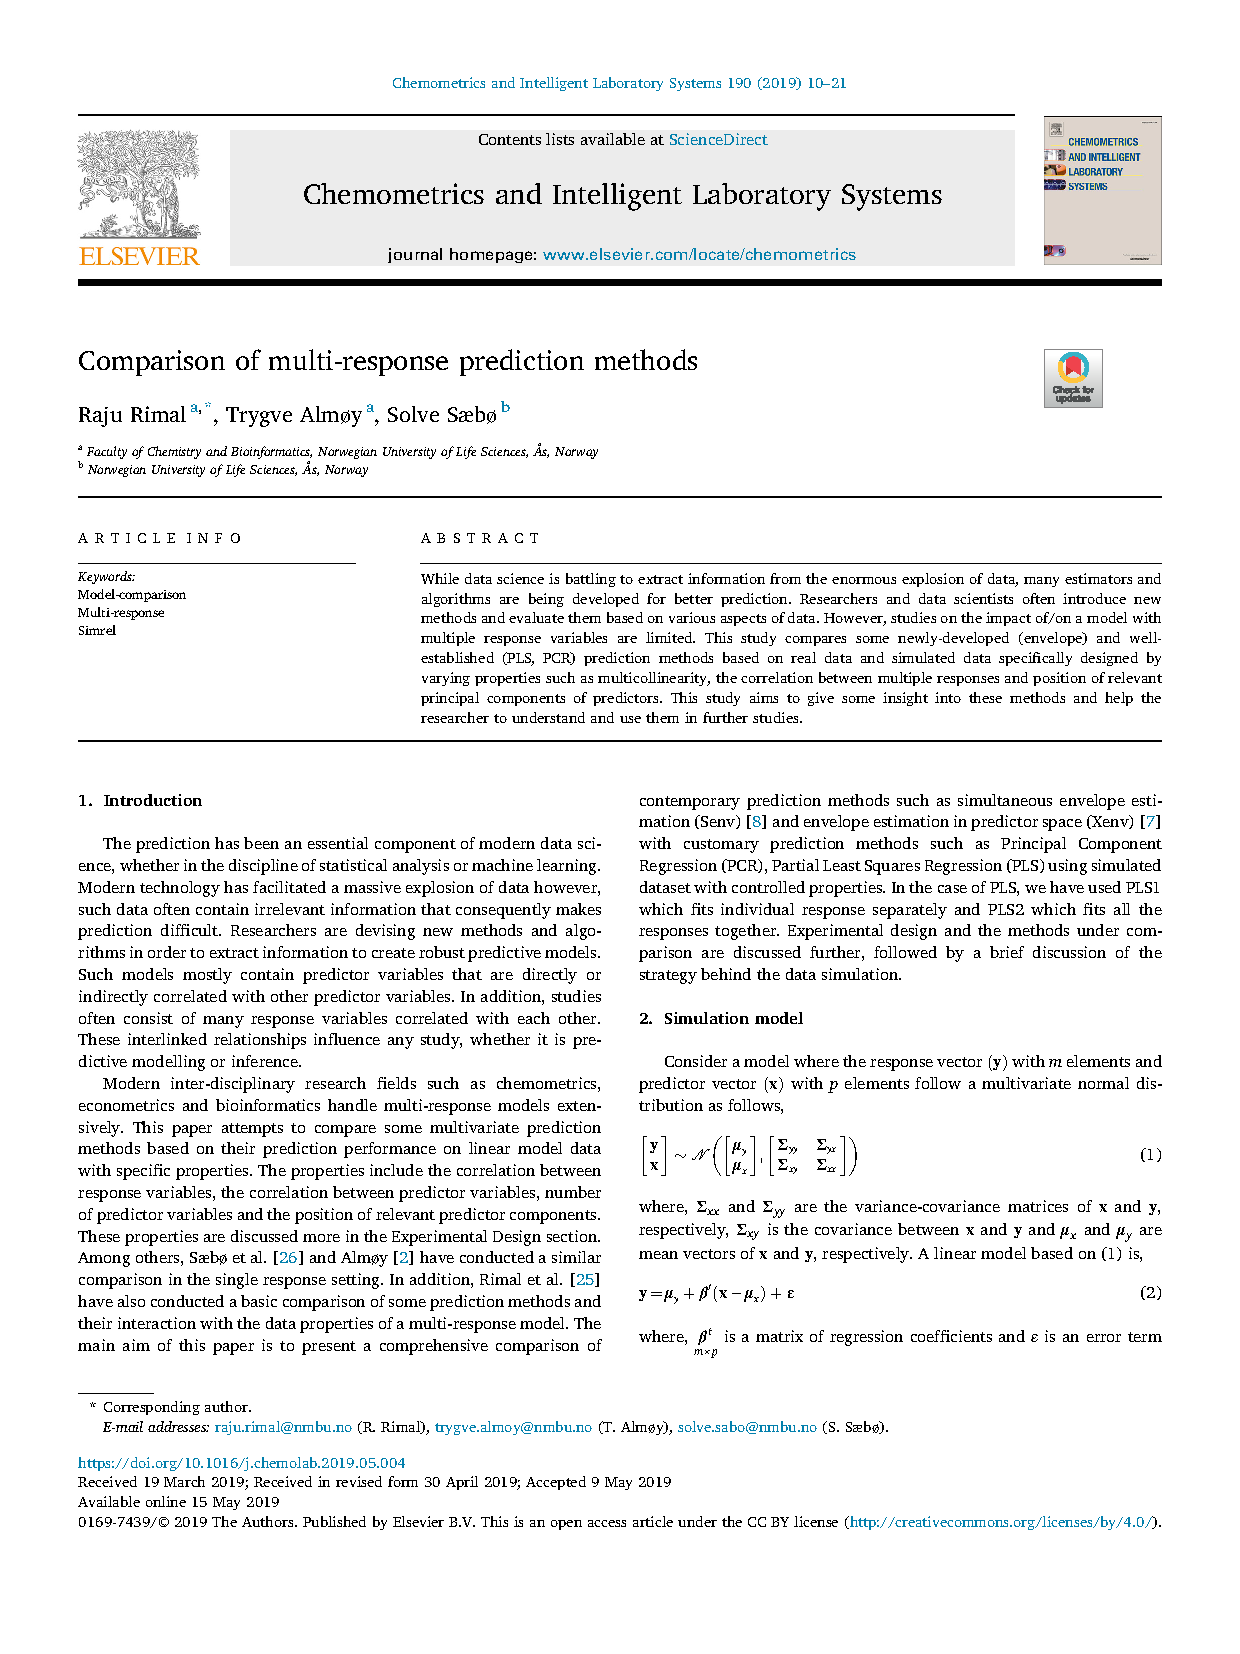
\includepdf[pages=-1]{papers/003.pdf}
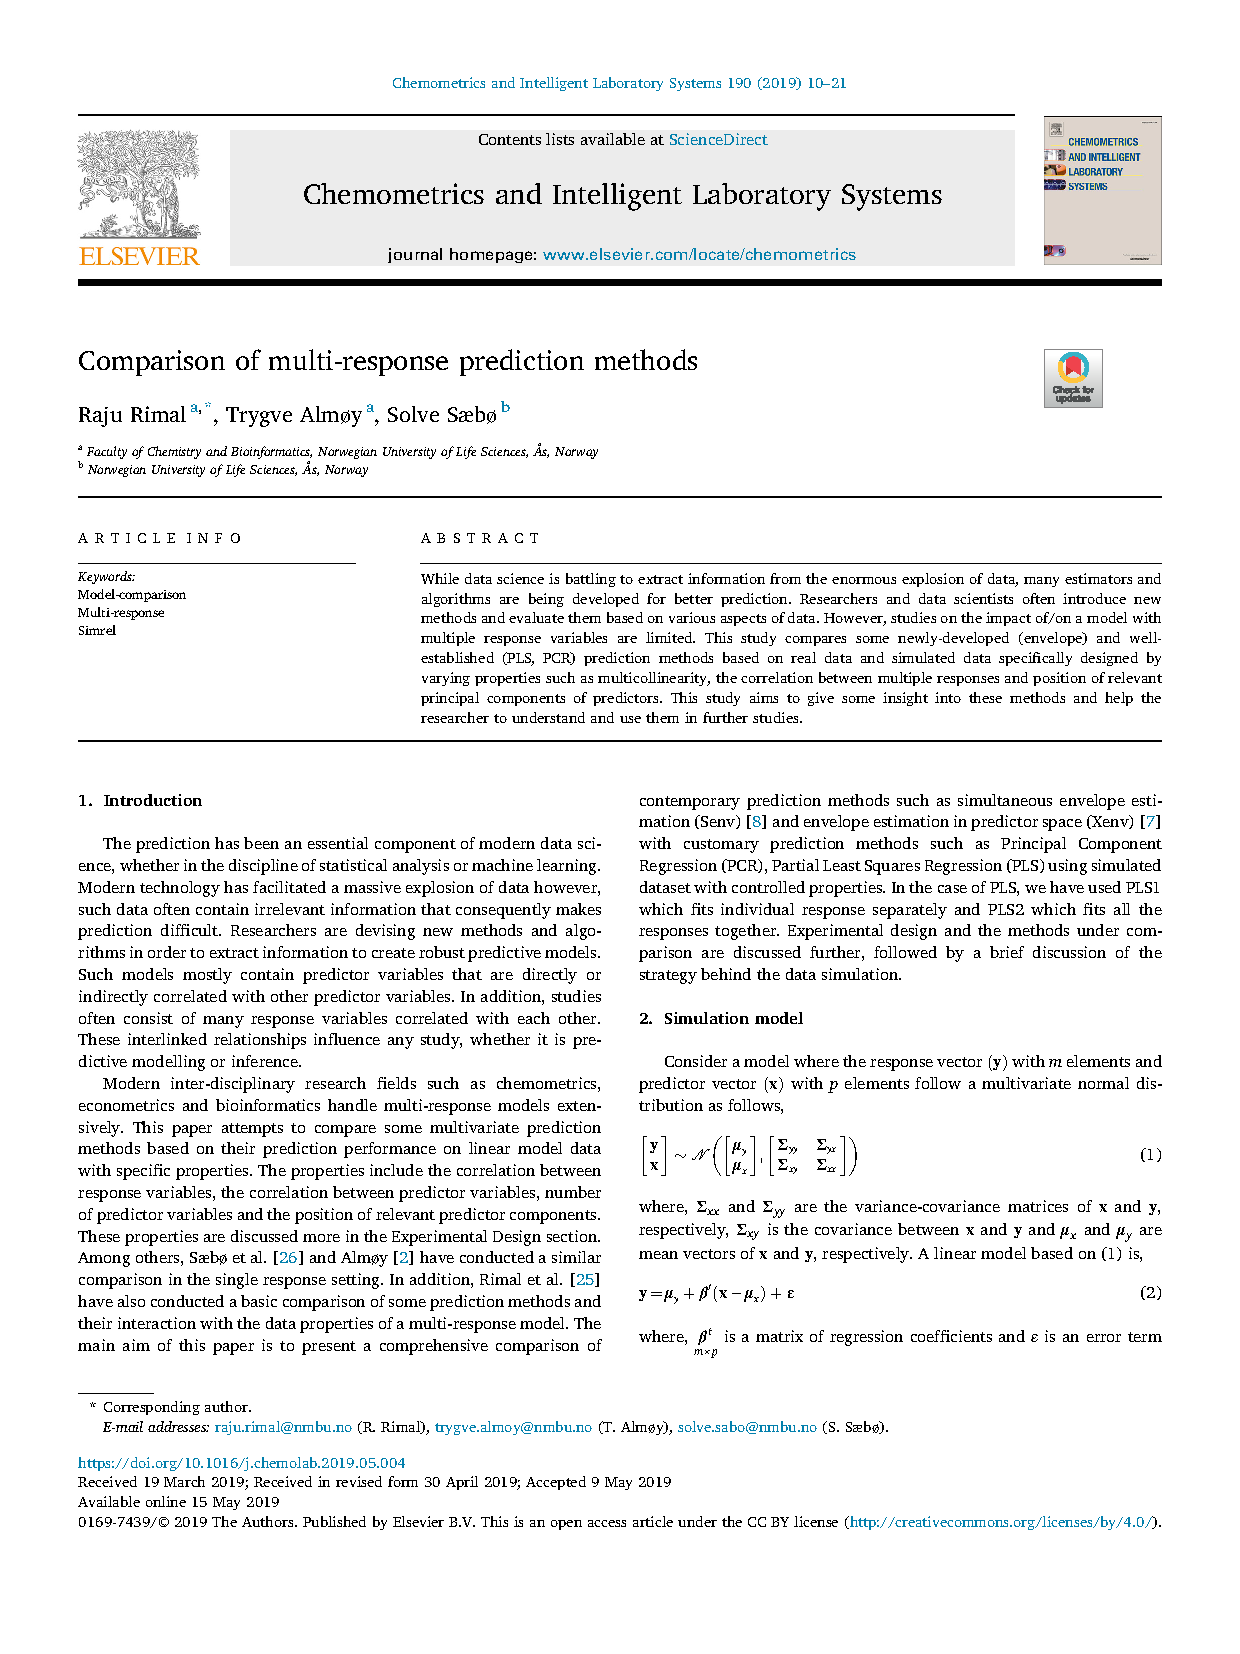
\includepdf[pages=-]{papers/003.pdf}
\par\chapter{Comparison of Multi-response Estimation Methods}
\cleardoublepage
%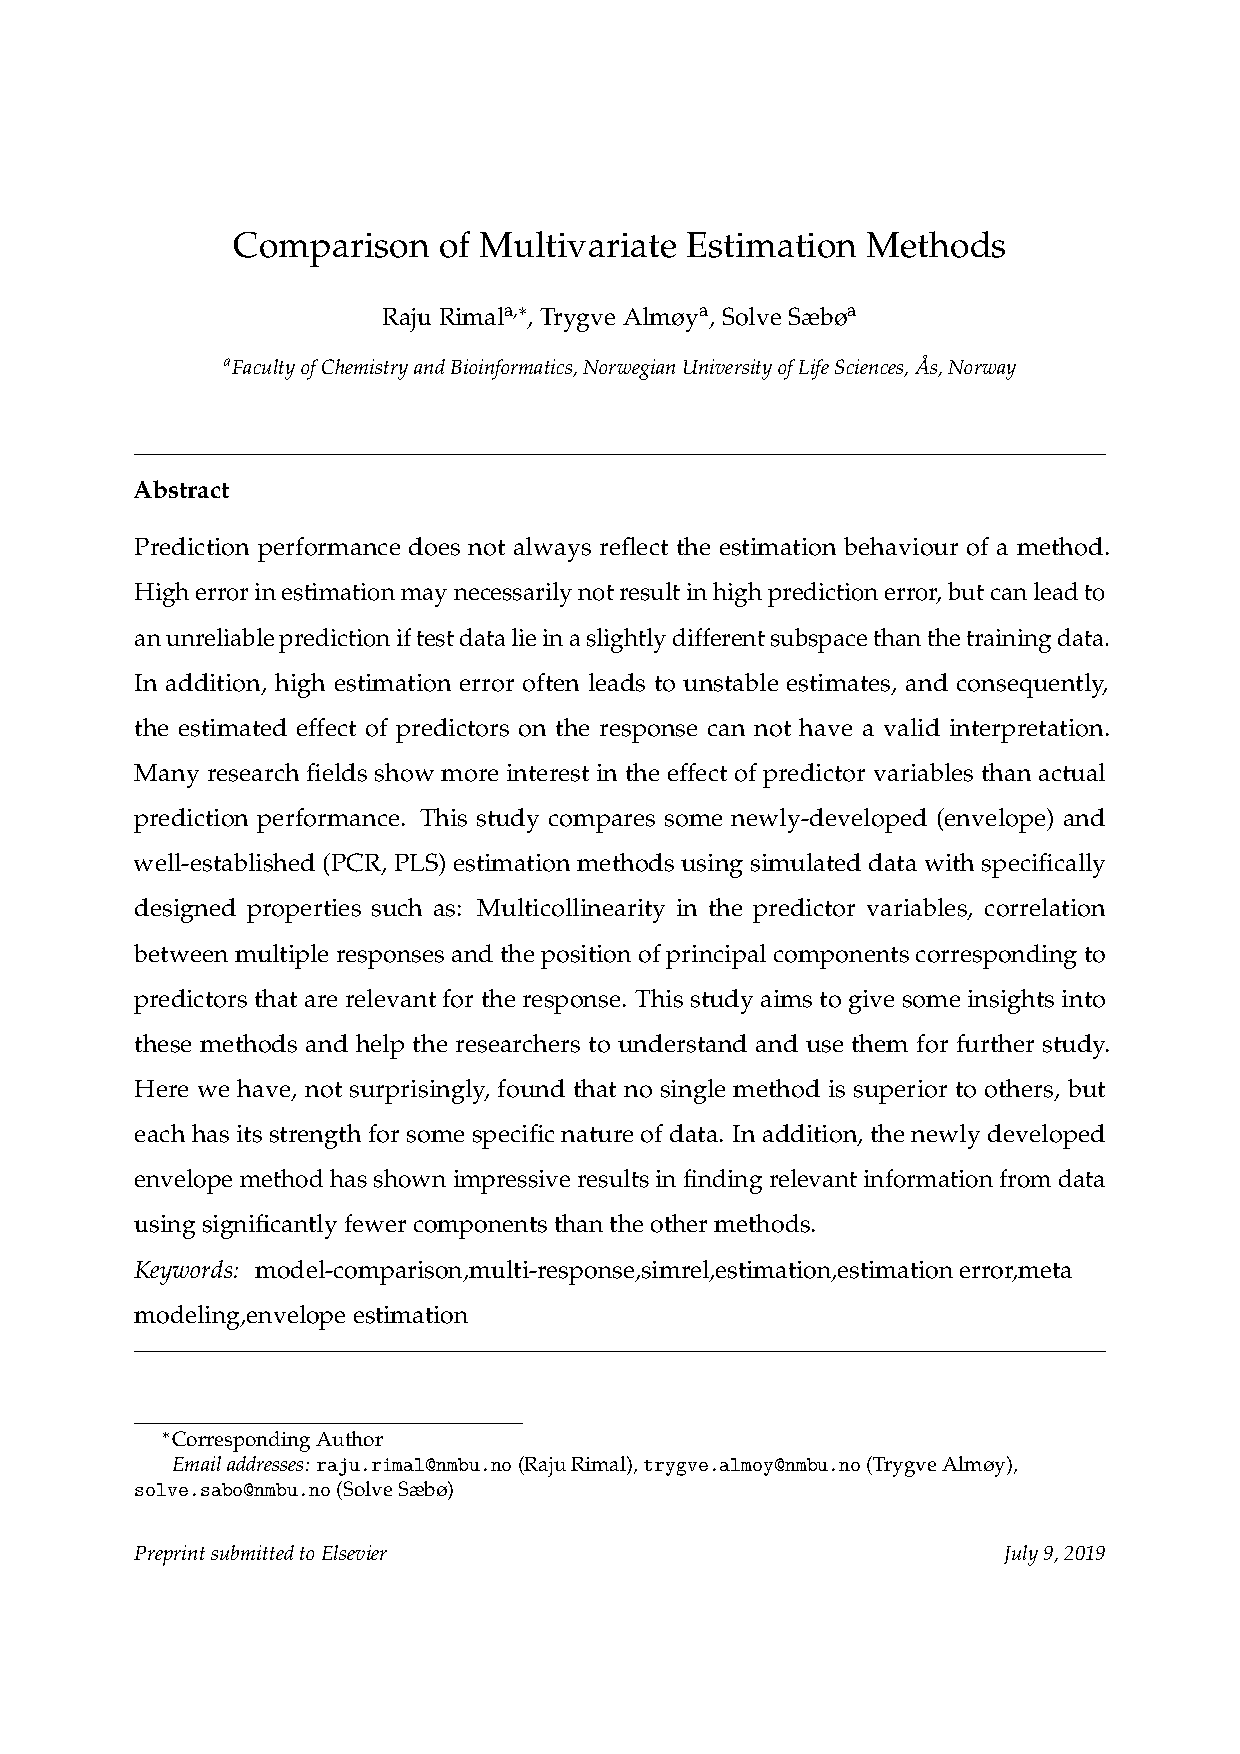
\includepdf[pages=-1]{papers/004.pdf}
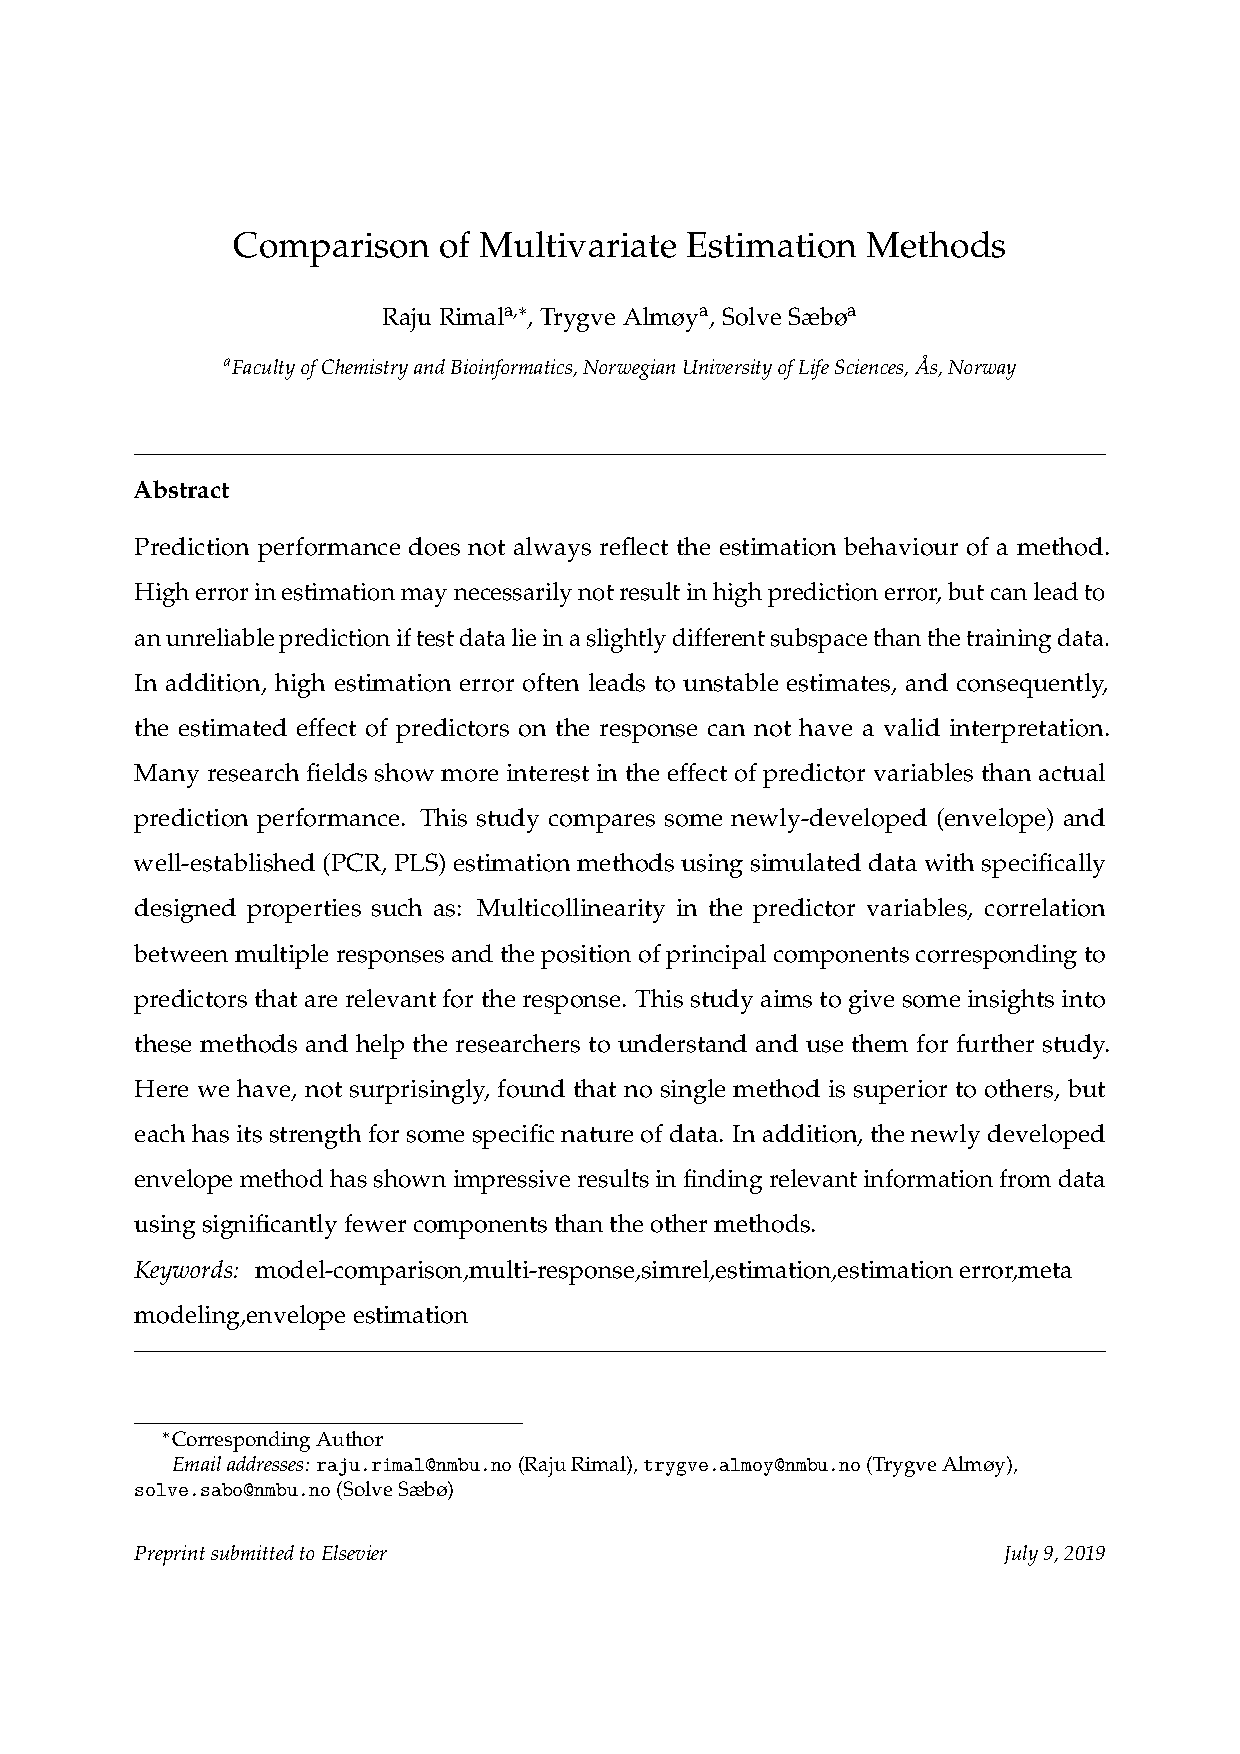
\includepdf[pages=-]{papers/004.pdf}

% *******************************************************
% ANYTHING EXTRA
% *******************************************************

\end{document}

%%% Local Variables:
%%% mode: latex
%%% TeX-master: t
%%% End:
